
\documentclass[journal,12pt,twocolumn]{IEEEtran}

\usepackage{graphicx}
\usepackage{setspace}
\usepackage{gensymb}
\singlespacing
\usepackage[cmex10]{amsmath}
\usepackage{amssymb}
\usepackage{xurl}
\usepackage{tabularx}
\usepackage{amsthm}
\usepackage{comment}
\usepackage{mathrsfs}
\usepackage{txfonts}
\usepackage{stfloats}
\usepackage{bm}
\usepackage{cite}
\usepackage{cases}
\usepackage{subfig}
\usepackage{arydshln}
\usepackage{longtable}
\usepackage{multirow}
\usepackage{amsmath}
\usepackage{enumitem}
\usepackage{mathtools}
\usepackage{steinmetz}
\usepackage{tikz}
\usepackage{circuitikz}
\usepackage{verbatim}
\usepackage{tfrupee}
\usepackage[breaklinks=true]{hyperref}
\usepackage{graphicx}
\usepackage{tkz-euclide}
\usetikzlibrary{automata, positioning}
\usetikzlibrary{calc,math}
\usepackage{listings}
    \usepackage{color}                                            %%
    \usepackage{array}                                            %%
    \usepackage{longtable}                                        %%
    \usepackage{calc}                                             %%
    \usepackage{multirow}                                         %%
    \usepackage{hhline}                                           %%
    \usepackage{ifthen}                                           %%
    \usepackage{lscape}     
\usepackage{multicol}
\usepackage{chngcntr}
\usepackage{blkarray}

\DeclareMathOperator*{\Res}{Res}

\renewcommand\thesection{\arabic{section}}
\renewcommand\thesubsection{\thesection.\arabic{subsection}}
\renewcommand\thesubsubsection{\thesubsection.\arabic{subsubsection}}

\renewcommand\thesectiondis{\arabic{section}}
\renewcommand\thesubsectiondis{\thesectiondis.\arabic{subsection}}
\renewcommand\thesubsubsectiondis{\thesubsectiondis.\arabic{subsubsection}}


\hyphenation{op-tical net-works semi-conduc-tor}
\def\inputGnumericTable{}                                 %%

\lstset{
%language=C,
frame=single, 
breaklines=true,
columns=fullflexible
}
\begin{document}


\newtheorem{theorem}{Theorem}[section]
\newtheorem{problem}{Problem}
\newtheorem{proposition}{Proposition}[section]
\newtheorem{lemma}{Lemma}[section]
\newtheorem{corollary}[theorem]{Corollary}
\newtheorem{example}{Example}[section]
\newtheorem{definition}[problem]{Definition}

\newcommand{\BEQA}{\begin{eqnarray}}
\newcommand{\EEQA}{\end{eqnarray}}
\newcommand{\define}{\stackrel{\triangle}{=}}
\bibliographystyle{IEEEtran}
\raggedbottom
\setlength{\parindent}{0pt}
\providecommand{\mbf}{\mathbf}
\providecommand{\pr}[1]{\ensuremath{\Pr\left(#1\right)}}
\providecommand{\qfunc}[1]{\ensuremath{Q\left(#1\right)}}
\providecommand{\sbrak}[1]{\ensuremath{{}\left[#1\right]}}
\providecommand{\lsbrak}[1]{\ensuremath{{}\left[#1\right.}}
\providecommand{\rsbrak}[1]{\ensuremath{{}\left.#1\right]}}
\providecommand{\brak}[1]{\ensuremath{\left(#1\right)}}
\providecommand{\lbrak}[1]{\ensuremath{\left(#1\right.}}
\providecommand{\rbrak}[1]{\ensuremath{\left.#1\right)}}
\providecommand{\cbrak}[1]{\ensuremath{\left\{#1\right\}}}
\providecommand{\lcbrak}[1]{\ensuremath{\left\{#1\right.}}
\providecommand{\rcbrak}[1]{\ensuremath{\left.#1\right\}}}
\theoremstyle{remark}
\newtheorem{rem}{Remark}
\newcommand{\sgn}{\mathop{\mathrm{sgn}}}
\providecommand{\abs}[1]{\vert#1\vert}
\providecommand{\res}[1]{\Res\displaylimits_{#1}} 

%\providecommand{\norm}[1]{\lVert#1\rVert}
\providecommand{\mtx}[1]{\mathbf{#1}}
\providecommand{\mean}[1]{E[ #1 ]}
\providecommand{\fourier}{\overset{\mathcal{F}}{ \rightleftharpoons}}
%\providecommand{\hilbert}{\overset{\mathcal{H}}{ \rightleftharpoons}}
\providecommand{\system}{\overset{\mathcal{H}}{ \longleftrightarrow}}
	%\newcommand{\solution}[2]{\textbf{Solution:}{#1}}
\newcommand{\solution}{\noindent \textbf{Solution: }}
\newcommand{\cosec}{\,\text{cosec}\,}
\providecommand{\dec}[2]{\ensuremath{\overset{#1}{\underset{#2}{\gtrless}}}}
\newcommand{\myvec}[1]{\ensuremath{\begin{pmatrix}#1\end{pmatrix}}}
\newcommand{\mydet}[1]{\ensuremath{\begin{vmatrix}#1\end{vmatrix}}}
\newcommand*{\permcomb}[4][0mu]{{{}^{#3}\mkern#1#2_{#4}}}
\newcommand*{\perm}[1][-3mu]{\permcomb[#1]{P}}
\newcommand*{\comb}[1][-1mu]{\permcomb[#1]{C}}
\numberwithin{equation}{subsection}
\makeatletter
\@addtoreset{figure}{problem}
\makeatother
\let\StandardTheFigure\thefigure
\let\vec\mathbf
\renewcommand{\thefigure}{\theproblem}
\def\putbox#1#2#3{\makebox[0in][l]{\makebox[#1][l]{}\raisebox{\baselineskip}[0in][0in]{\raisebox{#2}[0in][0in]{#3}}}}
     \def\rightbox#1{\makebox[0in][r]{#1}}
     \def\centbox#1{\makebox[0in]{#1}}
     \def\topbox#1{\raisebox{-\baselineskip}[0in][0in]{#1}}
     \def\midbox#1{\raisebox{-0.5\baselineskip}[0in][0in]{#1}}
\vspace{3cm}
\title{ ASSIGNMENT 5}
\author{HARITHA R\\ AI20BTECH11010}
\maketitle
\newpage
\bigskip
\newcommand\norm[1]{\left\lVert#1\right\rVert}

\renewcommand{\thefigure}{\arabic{figure}}
\renewcommand{\thetable}{\arabic{table}}
Download all python codes from
\begin{lstlisting}
https://github.com/harithar1234/EE3900-Haritha/blob/main/Assignment5/assignment5.py
\end{lstlisting}
\section*{QUESTION}
\textbf{Quadratic Forms/Q 2.8}
\begin{enumerate}
Find the area bounded by the curves  \\ 
$ \norm{\vec{x}-\myvec{1 \\0}} =1 $ and $\| \vec{x} \| =1 $ 
\end{enumerate}
\section*{SOLUTION}
\begin{enumerate}
General equation of circle is
\begin{align}
  \Vec{x}^\top\Vec{x} - 2 \Vec{O}^\top \Vec{x} + f=0
\end{align}
Taking equation of the first circle to be,
\begin{align}
 \norm{\vec{x}-\myvec{1 \\0}} ^2 =1 ^2   \\ 
 \Vec{x}^\top\Vec{x} - 2 \myvec{1&0} \Vec{x} + 1 =1\\
  \Vec{x}^\top\Vec{x} - 2 \myvec{1&0} \Vec{x}  =0 \label{eq:1}\\
\Vec{x}^\top\Vec{x} - 2 \Vec{O_1}^\top \Vec{x} + f_1=0\\
\Vec{O_1}=\myvec{1\\0}\\
f_1=0
\end{align}
Taking equation of the second circle to be,
\begin{align}
 \norm{\vec{x}} ^2 =1 ^2   \\ 
 \Vec{x}^\top\Vec{x} -1=0 \label{eq:2} \\
\Vec{x}^\top\Vec{x} - 2 \Vec{O_2}^\top \Vec{x} + f_2=0\\
\Vec{O_2}=\myvec{0\\0}\\
f_2=-1
\end{align}
substituting $\vec{O_2}$ in equation of first circle,
\begin{align}
     \norm{\vec{O_2}-\myvec{1 \\0}}=\norm{\myvec{0\\0}-\myvec{1 \\0}}  =1  
\end{align}
so $\vec{O_2}$ lies on first circle.\\
substituting $\vec{O_1}$ in equation of second circle,
\begin{align}
     \norm{\vec{O_1}}=\norm{\myvec{1 \\0}}  =1  
\end{align}
so $\vec{O_1}$ lies on second circle.
So each circle passes through the centre of the other.\\
Subtracting \eqref{eq:2} from \eqref{eq:1} we get the chord of intersection as,
\begin{align}
     \Vec{x}^\top\Vec{x} - 2 \myvec{1&0} \Vec{x} -\{\Vec{x}^\top\Vec{x} -1\} =0 -0\\
 \Vec{x}^\top\Vec{x} - 2 \myvec{1&0}\Vec{x} = \Vec{x}^\top\Vec{x} -1\\
- 2 \myvec{1&0}\Vec{x} = -1\\
\myvec{1&0}\Vec{x} = \frac{1}{2}
\end{align}
This can be written as,
\begin{align}
    \myvec{1&0}\Vec{x} = \frac{1}{2}=0.5\\
   \vec{x}=\myvec{0.5\\0}+\lambda\myvec{0\\1} \\
    \vec{x}=\vec{q}+\lambda\vec{m} \label{eq:3}\\
   \vec{q}=\myvec{0.5\\0}\\
   \vec{m}=\myvec{0\\1}
\end{align}
Substituting \eqref{eq:3} in \eqref{eq:2} we get
\begin{align}
 (\vec{q}+\lambda\vec{m})^\top (\vec{q}+\lambda\vec{m})-1=0\\
 \vec{q}^\top(\vec{q}+\lambda\vec{m})+\lambda\vec{m}^\top(\vec{q}+\lambda\vec{m})-1=0\\
 \vec{q}^\top\vec{q} +  \lambda\vec{q}^\top\vec{m} + \lambda\vec{m}^\top\vec{q} +  \lambda^2\vec{m}^\top\vec{m} -1=0\\
 \|\vec{q}\|^2 + 2\lambda\vec{q}^\top\vec{m} + \lambda^2\|\vec{m}\|^2 -1=0\\
  \|\vec{q}\|^2 + \lambda^2\|\vec{m}\|^2 -1=0 
\end{align}
 since $ \vec{q}^\top\vec{m}=0 $
\begin{align}
  \lambda^2= \frac{1- \|\vec{q}\|^2}{\|\vec{m}\|^2}\\
  \lambda^2=\frac{3}{4}\\
    \lambda= +\frac{\sqrt{3}}{2},-\frac{\sqrt{3}}{2}
\end{align}
Substituting the value of $\lambda$ in \eqref{eq:3} we get point of intersections of  the circles as
\begin{align}
   \vec{A}= \myvec{0.5\\+\frac{\sqrt{3}}{2}}\\
\vec{B}= \myvec{0.5\\-\frac{\sqrt{3}}{2}}
\end{align}
Now finding the direction vectors
\begin{align}
    \vec{m_{O_1A}}=\myvec{1\\0}-\myvec{0.5\\\frac{\sqrt{3}}{2}}=\myvec{0.5\\-\frac{\sqrt{3}}{2}}\\
     \vec{m_{O_1B}}=\myvec{1\\0}-\myvec{0.5\\-\frac{\sqrt{3}}{2}}=\myvec{0.5\\\frac{\sqrt{3}}{2}}\\
     \vec{m_{O_2A}}=\myvec{0\\0}-\myvec{0.5\\\frac{\sqrt{3}}{2}}=\myvec{-0.5\\-\frac{\sqrt{3}}{2}}\\
     \vec{m_{O_2B}}=\myvec{0\\0}-\myvec{0.5\\-\frac{\sqrt{3}}{2}}=\myvec{-0.5\\\frac{\sqrt{3}}{2}}\\
\end{align}
Finding the angle $\angle A O_1 B$
\begin{align}
\cos\theta_1 = \frac{ (\vec{m_{O_1A}})^\top \vec{m_{O_1B}} } { \|\vec{m_{O_1A}} \| \|\vec{m_{O_1B}}\|  }\\
\cos\theta_1 = \frac{-2}{4}=\frac{-1}{2}\\
\theta_1 = 120^{\circ} 
\end{align}
Finding the angle $\angle A O_2 B$
\begin{align}
\cos\theta_2 = \frac{ (\vec{m_{O_2A}})^\top \vec{m_{O_2B}} } { \|\vec{m_{O_2A}} \| \|\vec{m_{O_2B}}\|  }\\
\cos\theta_2 = \frac{-2}{4}=\frac{-1}{2}\\
\theta_2 = 120^{\circ} 
\end{align}
In general Area of a Segment in degrees is $ (\frac{\pi}{360}) \theta  r^2 -\frac{1}{2} r^2 \sin\theta $\\

The radius of $ \norm{\vec{x}} ^2 =1 ^2 $ is 1.\\
Area of a Segment $O_1 AB$ is
\begin{align} 
Area_{O_1 AB}= (\frac{\pi}{360})(120)(1^2) -\frac{1}{2}( 1^2) \sin (120)\\
Area_{O_1 AB}= \frac{\pi}{3} - \frac{1}{2}(\frac{\sqrt{3}}{2})
= \frac{\pi}{3} - \frac{\sqrt{3}}{4}
\end{align}

The radius of $ \norm{\vec{x}-\myvec{1 \\0}} ^2 =1 ^2 $ is 1.\\
Area of a Segment $O_2 AB$ is
\begin{align} 
Area_{O_2 AB}= (\frac{\pi}{360})(120)(1^2) -\frac{1}{2}( 1^2) \sin (120)\\
Area_{O_2 AB}= \frac{\pi}{3} - \frac{1}{2}(\frac{\sqrt{3}}{2})
= \frac{\pi}{3} - \frac{\sqrt{3}}{4}
\end{align}
Area of region bounded by curves is area of the region $O_1 A O_2 B $
\begin{align}
Area_{O_1 A O_2 B } =Area_{O_1 AB} + Area_{O_2 AB}= 2\cross (\frac{\pi}{3} - \frac{\sqrt{3}}{4})\\
Area_{O_1 A O_2 B } =\frac{2\pi}{3} - \frac{\sqrt{3}}{2}
\end{align}
\end{enumerate}
\begin{center}
    \huge{Area=$\frac{2\pi}{3} - \frac{\sqrt{3}}{2}$}
\end{center}

\begin{figure}[htp]
    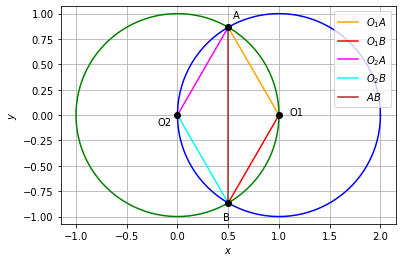
\includegraphics[scale=0.74]{figure_assignment5.png}
    \caption{plot}
\end{figure}
\end{document}